\documentclass[sigconf,review,anonymous]{acmart}

\usepackage{booktabs}
\usepackage{amsmath}

\settopmatter{printacmref=false}
\setcopyright{none}
\renewcommand\footnotetextcopyrightpermission[1]{}
\acmConference[SIGIR '27]{Proceedings of the 50th International ACM SIGIR Conference on Research and Development in Information Retrieval}{2027}{}

\newcommand{\gate}{$^\dagger$}

\begin{document}

\title{Stopping with Flow Networks: Chance Nodes, Risk Neutrality, and Technology-Assisted Review}

\author{Anonymous Author(s)}
\affiliation{\institution{Anonymous Institution}\country{}}

\begin{abstract}
Generative flow networks (GFlowNets) reach terminal states in proportion to a reward, which makes them an appealing way to learn when to stop screening in technology-assisted review (TAR). The obvious construction is wrong: a GFlowNet sums over every child, so it treats labels the reviewer has not yet seen as if the reviewer had chosen them. We keep flow matching at the reviewer's choices and aggregate chance nodes in log space. The resulting network obeys the soft Bellman equation of the belief MDP and is an ordinary GFlowNet when nothing is left to chance. On five toy problems it recovers the Bayes-optimal policy, where expected-flow and fixed-chain constructions do not. A TAR instance with reward-structured flows, soft policy iteration and prefix-only features matches the reliability of the IP-H point-process estimator on CLEF 2017--2019 at target recall 0.9 while reviewing 4.1 points less of each pool (95\% CI 1.3--6.9). That meets criteria fixed in advance, but only after four revisions on the same topics. On an external collection with much weaker rankings (SYNERGY) it does not beat the point-process rules. We report both.
\end{abstract}

\begin{CCSXML}
<ccs2012>
<concept><concept_id>10002951.10003317.10003359</concept_id><concept_desc>Information systems~Evaluation of retrieval results</concept_desc><concept_significance>500</concept_significance></concept>
<concept><concept_id>10010147.10010257.10010258.10010261</concept_id><concept_desc>Computing methodologies~Reinforcement learning</concept_desc><concept_significance>300</concept_significance></concept>
</ccs2012>
\end{CCSXML}
\ccsdesc[500]{Information systems~Evaluation of retrieval results}
\ccsdesc[300]{Computing methodologies~Reinforcement learning}
\keywords{Technology-assisted review, stopping rules, generative flow networks}

\maketitle

\section{Introduction}

In technology-assisted review (TAR), a reviewer screens a ranked pool of documents until enough of the relevant ones have been found. A \emph{stopping rule} decides when to stop. It should reach a target recall on almost every topic while screening as little of the pool as possible. Existing rules are heuristics on the gain curve~\cite{cormack2016engineering,yang2021heuristic}, estimators of the relevant documents that remain~\cite{sneyd2019modelling,stevenson2023point,callaghan2020statistical,li2020stop}, sampling certificates~\cite{lewis2021certifying}, and learned policies~\cite{binhezam2024rlstop}.

Generative flow networks (GFlowNets)~\cite{bengio2021flow,bengio2023foundations,malkin2022trajectory} learn a forward policy that reaches each terminal state in proportion to a reward. Stopping seems a natural fit: the terminal states are stopping points and the reward trades review cost against missed recall. A stopping problem, however, contains \emph{chance nodes}. After the reviewer continues, the next label is revealed. After the reviewer stops, the documents not yet seen decide whether the target was met. A GFlowNet built on each realised ranking treats those outcomes as choices. Expected flow networks~\cite{jiralerspong2024expected} add chance nodes but average flows arithmetically, which we show is risk-seeking for stopping.

\textbf{Contributions.}
(1)~A flow network for stopping whose chance nodes are aggregated in log space. It is the soft Bellman equation of the belief MDP, recovers the Bayes policy as the temperature falls, and is an ordinary GFlowNet when nothing is left to chance. We contrast it, exactly, with the fixed-chain and expected-flow constructions.
(2)~A learned TAR instance. Its flows are parameterised by the reward's structure and trained by soft policy iteration on realised rankings, from features computed only on the reviewed prefix.
(3)~An evaluation on CLEF 2017--2019 and on SYNERGY against rules replayed in one framework, judged by criteria fixed in advance, with ablations and negative results.

\section{Stopping Flow Networks}

Let $h$ be the labels seen so far. At a \emph{reviewer node} the reviewer chooses \texttt{continue} or a terminal action $a$. A \emph{chance node} follows each choice: \texttt{continue} reveals the next label $y\sim p(y\mid h)$, and $a$ meets a latent world $w\sim p(w\mid h)$ that fixes the utility $U(h,a,w)$. Terminal flows are rewards, $F=R=\exp(\beta U)$. At reviewer nodes we keep the GFlowNet constraints $F(h)=\sum_a F(h,a)$ and $P_F(a\mid h)=F(h,a)/F(h)$. Three ways of aggregating a chance node's children give three networks:
\emph{hindsight}: sum within each realised chain (the fixed-chain GFlowNet), then average over chains;
\emph{arithmetic}: $F(h,a)=\mathbb{E}[F(\mathrm{child})\mid h]$, as in expected flow networks~\cite{jiralerspong2024expected};
\emph{geometric} (ours): $\log F(h,a)=\mathbb{E}[\log F(\mathrm{child})\mid h]$.
In value units $Q=\log F/\beta$, the geometric network gives $Q(h,a)=\mathbb{E}[U\mid h,a]$ for terminal actions and $Q(h,\texttt{continue})=\mathbb{E}_y[V(hy)]$, with $V(h)=\beta^{-1}\log\sum_a e^{\beta Q(h,a)}$: the soft Bellman equation~\cite{haarnoja2017energy} of the belief MDP.

\textbf{Properties.} On a finite tree:
(a)~if $p$ is a point mass, all three coincide with a tree GFlowNet~\cite{bengio2021flow}, so terminals are reached in proportion to $R$; on trees this is entropy-regularised RL~\cite{tiapkin2024entropy};
(b)~the geometric network's greedy policy tends to the Bayes-optimal policy as $\beta\to\infty$;
(c)~$Q_{\mathrm{hind}}(h,\texttt{continue})\ge Q_{\mathrm{geo}}(h,\texttt{continue})$ for every $h$, by Jensen's inequality on the convex log-sum-exp applied from the leaves up, so hindsight overvalues continuing;
(d)~$Q_{\mathrm{arith}}(h,a)\to\max_w U(h,a,w)$ as $\beta\to\infty$, so the expected-flow network is risk-seeking.
Table~\ref{tab:toys} computes all three exactly on five toy laws over label sequences. The geometric network attains the Bayes value on all five. The arithmetic network collapses: with one label that reveals the world, it guesses at once instead of paying to look. The hindsight network falls short wherever looking ahead has value.

\begin{table}[t]
\caption{Exact expected utility of each network's greedy policy at $\beta=10^5$ on five toy laws ($L$ labels, threshold decision).}
\label{tab:toys}
\small
\setlength{\tabcolsep}{3.5pt}
\begin{tabular}{lcccc}
\toprule
Law & Bayes & Geometric & Hindsight & Arithm. \\
\midrule
Perfect information ($L{=}1$) & 0.240 & 0.240 & 0.240 & 0.000 \\
Beta-binomial ($L{=}8$) & 0.137 & 0.137 & 0.134 & 0.040 \\
Delayed information ($L{=}10$) & 0.178 & 0.178 & 0.177 & 0.008 \\
Clustered HMM ($L{=}10$) & 0.179 & 0.179 & 0.179 & 0.021 \\
Rank-decay mixture ($L{=}10$) & 0.188 & 0.188 & 0.186 & 0.063 \\
\bottomrule
\end{tabular}
\end{table}

\textbf{Learning from realised rankings.} Without a known law, terminal values are regressed on realised utilities, and the squared loss makes them conditional expectations, as the geometric chance node requires. The continue value cannot be regressed on a ranking's own future, since that is the hindsight target. A one-step soft backup through a frozen copy, as in fitted Q iteration, compounded noise over 200 checkpoints, and its continue values exceeded every attainable utility. We instead use \emph{soft policy iteration}. Each round evaluates the frozen forward policy exactly along every realised ranking and regresses the continue value on the value at the next checkpoint. The target averages only over the policy's own choices, which depend on observed features alone. It therefore carries neither hindsight nor maximisation bias, and its fixed point satisfies the geometric constraints. On an exchangeable toy, a network learned this way reaches the Bayes value to within 0.002.

\section{A Stopping Flow Network for TAR}

Stopping after $n$ of $N$ documents at target recall $\tau$ with miss penalty $\lambda$ earns $U=-\big(n/N+\lambda\,[\mathrm{recall}(n)<\tau]\big)/(1+\lambda)$. Both $\tau$ and $\lambda$ are inputs, so one network serves every operating point. The flows follow the reward's structure:
\begin{align*}
\tfrac{1}{\beta}\log F(x,\texttt{stop}) &= -\big(n/N+\lambda\,\hat p(x)\big)/(1+\lambda),\\
\tfrac{1}{\beta}\log F(x,\texttt{cont}) &= -\big(c(x)+\lambda\,m(x)\big)/(1+\lambda)+e(x).
\end{align*}
Here $\hat p$ classifies whether the target is still unmet and does not see $\lambda$; we call the resulting rule GFlowStop. The terms $c$, $m$ and $e$ are the review fraction, miss probability and entropy bonus still to come under the current policy, with $c$ bounded below by the next checkpoint's review.

Stops are allowed at 200 evenly spaced checkpoints. Each state $x$ is computed from the reviewed prefix only, and a test flips every later label to check this. It contains the review fraction, documents found, precision, relevance rates over recent windows, and the gap since the last relevant document and how surprising it is. It also contains remaining-count estimates from window rates and from Poisson exponential and power-law fits, together with the latest state of the IP-H estimator~\cite{stevenson2023point} with the model tail: whether its fit was accepted, its estimated and Poisson-bound recall, an empty-tail flag and the fit's age. Each recall estimate also enters as its log-odds margin from $\tau$.

Training uses the AutoTAR rankings of the training collections, the 2017 and 2018 CLEF participant runs (48 runs, weight $0.25$) of years other than the test year, and eight thinned sub-pools of every AutoTAR ranking. A sub-pool keeps each relevant document with probability $U(0.6,1)$ and each other document with probability $e^{U(\log 0.1,0)}$, which yields smaller, denser rankings. Ten members (MLP heads $2\times64$, $\beta=10^4$, 120 rounds of 25 AdamW steps) each train on 70\% of the training topics. Out of bag, every training topic is scored by the members that never saw it. On those scores we choose, per target, the smallest penalty (grid $0.25$--$256$) from which reliability stays at or above $0.975$. We also choose between averaging the members' flows and stopping only when the least willing member would stop.

\section{Experimental Setup}

\textbf{CLEF.} The CLEF TAR collections of 2017, 2018 and 2019~\cite{kanoulas2017clef,kanoulas2018clef,kanoulas2019clef} have released AutoTAR rankings~\cite{stevenson2023point}: 91 topics (30, 30 and 31), plus 12 further 2017 topics used only for training. For 2017 we use the AutoStop qrels~\cite{li2020stop}, which the rankings match (with CLEF's training qrels, seven 2017 topics put every relevant document at the end of the ranking); 2018 and 2019 use the official abstract qrels. The oracle needs 5.7\%, 6.7\% and 7.1\% review to reach recall 0.9. We hold out one collection at a time and train on the rest.

\textbf{SYNERGY (external).} SYNERGY~\cite{debruin2023synergy} has 26 systematic reviews, 169{,}288 records and 2{,}834 inclusions. It ships no rankings, so we simulate AutoTAR~\cite{cormack2015autonomy}: TF-IDF logistic regression seeded with the review title, 100 random pseudo-negatives per round, and batches growing by a tenth. The oracle needs 27.7\% review to reach recall 0.9, four times CLEF's figure. SYNERGY played no part in development, and its protocol was recorded before any SYNERGY result.

\textbf{Baselines and measures.} A PyTerrier~\cite{macdonald2020pyterrier} extension for replaying stopping rules (anonymised) runs every rule on identical trajectories: the IP-H estimator with the released and the model tail, its Cox variant CX-H, IP-E and IP-P~\cite{stevenson2023point}; CMH~\cite{callaghan2020statistical}; Kneedle and Budget~\cite{cormack2016engineering}; ConsecutiveIrrelevant and BatchPrecision~\cite{yang2021heuristic}; and RLStop~\cite{binhezam2024rlstop} trained on the same topics. For $\tau\in\{0.8,0.9,0.95\}$ we report \emph{reliability}, the share of topics reaching $\tau$, and mean \emph{review}, the share of each pool screened. The gate, fixed before the first CLEF run, says rule $A$ beats $B$ at $\tau$ if $A$'s mean review is lower, with a paired topic-bootstrap 95\% interval below zero, and its reliability is at least $B$'s.

\section{Results}

\begin{table}[t]
\caption{CLEF 2017--2019, leave one collection out, 91 topics. Cells give reliability / review (\%). \gate: the final GFlowStop beats this rule at this target under the gate.}
\label{tab:clef}
\small
\setlength{\tabcolsep}{4pt}
\begin{tabular}{lccc}
\toprule
Rule & $\tau=0.8$ & $\tau=0.9$ & $\tau=0.95$ \\
\midrule
GFlowStop (final) & 98.9 / 10.3 & 97.8 / 14.4 & 97.8 / 17.2 \\
\quad without IP-H state & 97.8 / \phantom{0}9.8 & 96.7 / 12.9 & 96.7 / 19.0 \\
\quad first declared version & 96.7 / 13.1 & 95.6 / 19.7 & 95.6 / 32.2 \\
RLStop & 62.6 / \phantom{0}6.6 & 65.9 / \phantom{0}9.1 & 73.6 / 11.2 \\
IP-H, model tail & 100 / 17.6 & 97.8 / 18.5\gate & 97.8 / 20.0 \\
IP-H, released & 93.4 / 16.1\gate & 90.1 / 16.8 & 89.0 / 18.1 \\
CX-H & 93.4 / 17.8\gate & 91.2 / 19.0\gate & 87.9 / 19.9 \\
IP-E & 98.9 / 17.1\gate & 95.6 / 18.0\gate & 94.5 / 19.4 \\
IP-P & 100 / 27.7 & 100 / 28.6 & 100 / 28.9 \\
ConsecutiveIrrelevant & 100 / 20.8 & 97.8 / 20.8\gate & 95.6 / 20.8 \\
BatchPrecision & 100 / 31.5 & 98.9 / 31.5 & 96.7 / 31.5\gate \\
CMH & 100 / 47.6 & 100 / 60.8 & 100 / 72.3 \\
Oracle (offline) & 100 / \phantom{0}5.1 & 100 / \phantom{0}6.5 & 100 / \phantom{0}7.8 \\
\bottomrule
\end{tabular}
\end{table}

\begin{figure}[t]
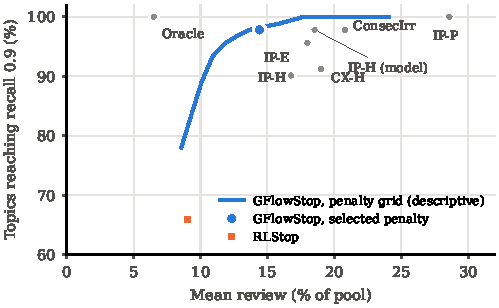
\includegraphics[width=\columnwidth]{frontier.pdf}
\caption{CLEF at $\tau=0.9$. The line is the final model at each fixed penalty (descriptive: picking a point on it would use test labels). The dot is the penalty chosen out of bag.}
\label{fig:frontier}
\end{figure}

\textbf{CLEF.} Table~\ref{tab:clef} and Figure~\ref{fig:frontier} give the results. At $\tau=0.9$ the final model matches the reliability of IP-H with the model tail (97.8\%) and reviews 4.1 points less (95\% CI $[-6.9,-1.3]$). Its reliability is the same in every collection (100\%, 93.3\%, 100\%), and its review is lower in each (14.7, 13.2 and 15.3\% against 16.3, 17.4 and 21.7\%). It also passes the gate against IP-E, CX-H and ConsecutiveIrrelevant at 0.9, against the released IP-H, CX-H and IP-E at 0.8, and against BatchPrecision at 0.95. Two comparisons are trade-offs rather than wins. At 0.8 it reviews 7.3 points less than IP-H with the model tail but misses one more topic. At 0.95 it has the same reliability and reviews 2.8 points less, but the interval $[-6.1,+0.7]$ includes zero. IP-P, which reaches every topic at 28--29\% review, is never beaten. RLStop trained on the same topics stops early and reaches the target on only 63--74\% of topics. The IP-H state adds one topic at every target over an otherwise identical network.

The first declared version (Table~\ref{tab:clef}) failed the gates. Four revisions followed, each recorded before its run: tail-fit features, thinned sub-pools, the bagged ensemble with out-of-bag selection, and the IP-H state. All were evaluated on the same 91 topics, so the CLEF results are not an independent confirmation.

\textbf{What matters.} Table~\ref{tab:ablation} varies only the continue target. A one-step lookahead never exceeds 65\% reliability at any penalty, so looking further ahead is essential. Hard ($\beta=\infty$) and soft policy iteration are indistinguishable, so the GFlowNet's sampling temperature adds nothing at this scale. The hindsight target continues longer at every penalty, as property~(c) predicts. Because the penalty is a free knob, its frontier is not uniformly worse: worse at 95\%, better near 100\%. What the risk-neutral construction buys is a penalty that keeps its meaning as the cost of a miss. Choosing the penalty from $k\le8$ labelled topics of each test collection, instead of out of bag, was less reliable with the same networks (93.7\% against 95.6\% at $\tau=0.9$, $k=8$).

\begin{table}[t]
\caption{Continue targets on CLEF at $\tau=0.9$ (single-seed networks without IP-H state). Least mean review (\%) on the penalty grid reaching each reliability, and the best reliability reached.}
\label{tab:ablation}
\small
\setlength{\tabcolsep}{4pt}
\begin{tabular}{lccc}
\toprule
Continue target & $\ge$95\% & $\ge$97.8\% & Best \\
\midrule
Geometric, soft policy iteration ($\beta{=}10^4$) & 17.1 & 25.3 & 98.9 \\
Geometric, hard ($\beta{=}\infty$) & 15.2 & 26.1 & 98.9 \\
Hindsight (best future stop of each chain) & 20.2 & 23.7 & 100 \\
One-step lookahead & -- & -- & 50.5 \\
\bottomrule
\end{tabular}
\end{table}

\begin{table}[t]
\caption{SYNERGY, 26 reviews, simulated AutoTAR rankings. Cells give reliability / review (\%).}
\label{tab:synergy}
\small
\setlength{\tabcolsep}{4pt}
\begin{tabular}{lccc}
\toprule
Rule & $\tau=0.8$ & $\tau=0.9$ & $\tau=0.95$ \\
\midrule
GFlowStop, trained on CLEF & 88.5 / 31.1 & 88.5 / 57.3 & 88.5 / 68.5 \\
\quad without IP-H state & 73.1 / 20.8 & 80.8 / 39.4 & 96.2 / 75.0 \\
GFlowStop, + in-domain folds & 100 / 48.5 & 96.2 / 78.1 & 96.2 / 79.1 \\
RLStop, trained on CLEF & 15.4 / \phantom{0}1.7 & \phantom{0}3.8 / \phantom{0}2.4 & 11.5 / \phantom{0}4.3 \\
IP-H, model tail & 92.3 / 34.2 & 84.6 / 35.6 & 80.8 / 39.2 \\
IP-H, released & 84.6 / 31.0 & 73.1 / 31.4 & 69.2 / 33.5 \\
IP-E & 88.5 / 33.4 & 76.9 / 34.4 & 73.1 / 36.6 \\
IP-P & 92.3 / 47.6 & 88.5 / 50.6 & 84.6 / 52.7 \\
ConsecutiveIrrelevant & 73.1 / 27.6 & 57.7 / 27.6 & 53.8 / 27.6 \\
Budget & 100 / 53.3 & 88.5 / 53.3 & 88.5 / 53.3 \\
CMH & 100 / 55.7 & 100 / 70.7 & 100 / 81.9 \\
Oracle (offline) & 100 / 19.7 & 100 / 27.7 & 100 / 32.5 \\
\bottomrule
\end{tabular}
\end{table}

\textbf{SYNERGY.} Table~\ref{tab:synergy} shows that, trained on CLEF, GFlowStop beats none of the point-process rules on these much weaker rankings. It is cheaper but less reliable than IP-H at 0.8, and over-cautious at 0.9 and 0.95. RLStop trained on CLEF collapses there. Adding the other folds' reviews to training (five folds, penalty chosen out of bag on in-domain reviews) improves the network itself. At a fixed penalty of 4 it reaches 92.3\% at 32.2\% review at 0.8, against 92.3\% at 34.2\% for IP-H with the model tail. Choosing the penalty on about 21 in-domain reviews, however, tolerates no miss, which forces cautious penalties. At $\tau=0.8$ it then matches CMH's 100\% with 7.2 points less review, but with 26 reviews the interval $[-16.1,+2.0]$ includes zero. Its only gate win is over Kneedle. Choosing the CLEF-trained network's penalty from $k\le8$ labelled SYNERGY reviews was never both cheaper and as reliable as IP-H with the model tail in 200 random draws.

\section{Discussion and Conclusion}

Posing stopping as a flow network is sound only if the chance nodes are aggregated risk-neutrally. Summing over them, the fixed-chain GFlowNet, prices continuing with hindsight. Averaging their flows, the expected-flow network, is risk-seeking. The corrected network is the soft Bellman equation, so a GFlowNet buys Bayes-consistent stopping and an interpretable miss penalty. In our experiments the entropy term contributed nothing beyond that. In practice the learned rule is only as good as its training distribution and its operating point. With the IP-H state as an input, it meets IP-H's reliability with less review on CLEF at recall 0.9. It does not carry that advantage to a collection whose rankings are four times weaker. There, per-ranking point-process estimators, which need no training, travel better.

\textbf{Limitations.} CLEF was used for five configurations. One CLEF topic is worth 1.1 points of reliability and one SYNERGY review 3.8, so many differences are within noise. The SYNERGY rankings are simulated. Reliability is measured, not certified.

\textbf{Reproducibility.} Code, configurations, per-topic stops, data provenance and the dated record of every revision are released (anonymised for review).

\bibliographystyle{ACM-Reference-Format}
\bibliography{references}

\end{document}
